\chapter[Resultados]{Resultados}

A partir do estudo e pesquisa realizado até o momento determinamos o que utilizar no conjunto do sistema, levantando um perfil que a equipe acredita ser a mais viável em termos de interação, custo-benefício, tempo, conhecimento técnico e outros fatores importantes para o projeto. Será desenvolvido um kit com capacidade de ser acoplado em diversas cadeiras de rodas afim de facilitar a mobilidade elétrica em cadeiras manuais. Os resultados levantados estão disposto no decorrer do capítulo.

\section{Estrutura}

Com a utilização do programa CATIA V5 3D foi estruturado o sistema eletrônico acoplado à cadeira de rodas, \ref{fig:vista_isometrica_traseira}. Visando três preceitos básicos: comodidade, acessibilidade e conforto.

\begin{figure}[!htb]
\centering
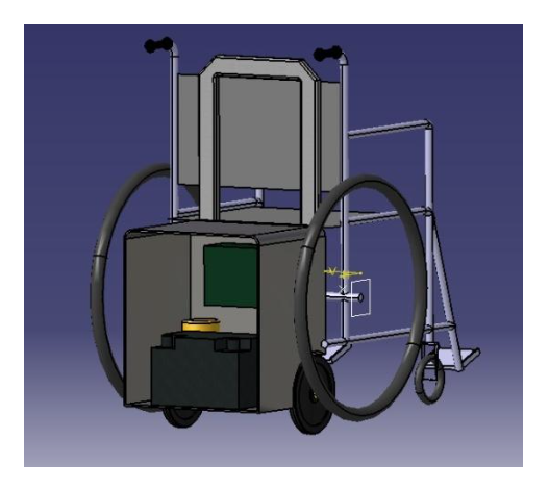
\includegraphics[keepaspectratio=true,scale=0.4]{figuras/estrutura/vista_isometrica_traseira}
\caption{Vista Isométrica Traseira}
\label{fig:vista_isometrica_traseira}
\end{figure}

O objetivo do projeto é desenvolver uma estrutura de fácil conexão e resistente. O produto proposto, ver figura \ref{fig:traseira},\ref{fig:sistema}, \ref{fig:lateral} e \ref{fig:superior},deve-se acoplar a qualquer cadeira de rodas. Foi pensado em um dispositivo no formato de uma mala para que seja de fácil conexão, uso e manuseio.

\begin{figure}[!htb]
\centering
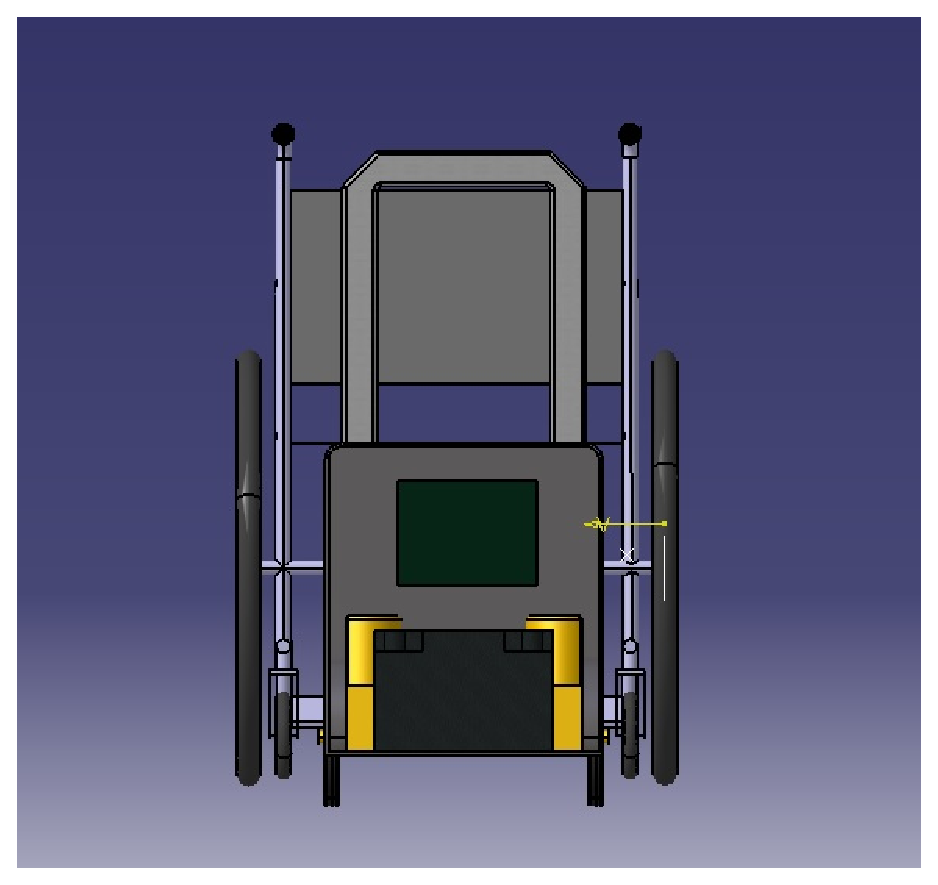
\includegraphics[keepaspectratio=true,scale=0.4]{figuras/estrutura/vista_traseira}
\caption{Vista Traseira}
\label{fig:traseira}
\end{figure}

A forma como a mala será acoplada a cadeira usa como base as hastes da mala e as hastes verticais aonde as manoplas utilizadas para empurrar manualmente a cadeira são fixadas. Tendo em vista que são rígidas e normatizadas pela NBR 9050 as hastes verticais da cadeira tem a distancia e espessura já definidas, o que facilita o desenvolvimento de um produto que possa ser usado em qualquer cadeira de rodas que esteja dentro dos padrões impostos pela norma.

\begin{figure}[!htb]
\centering
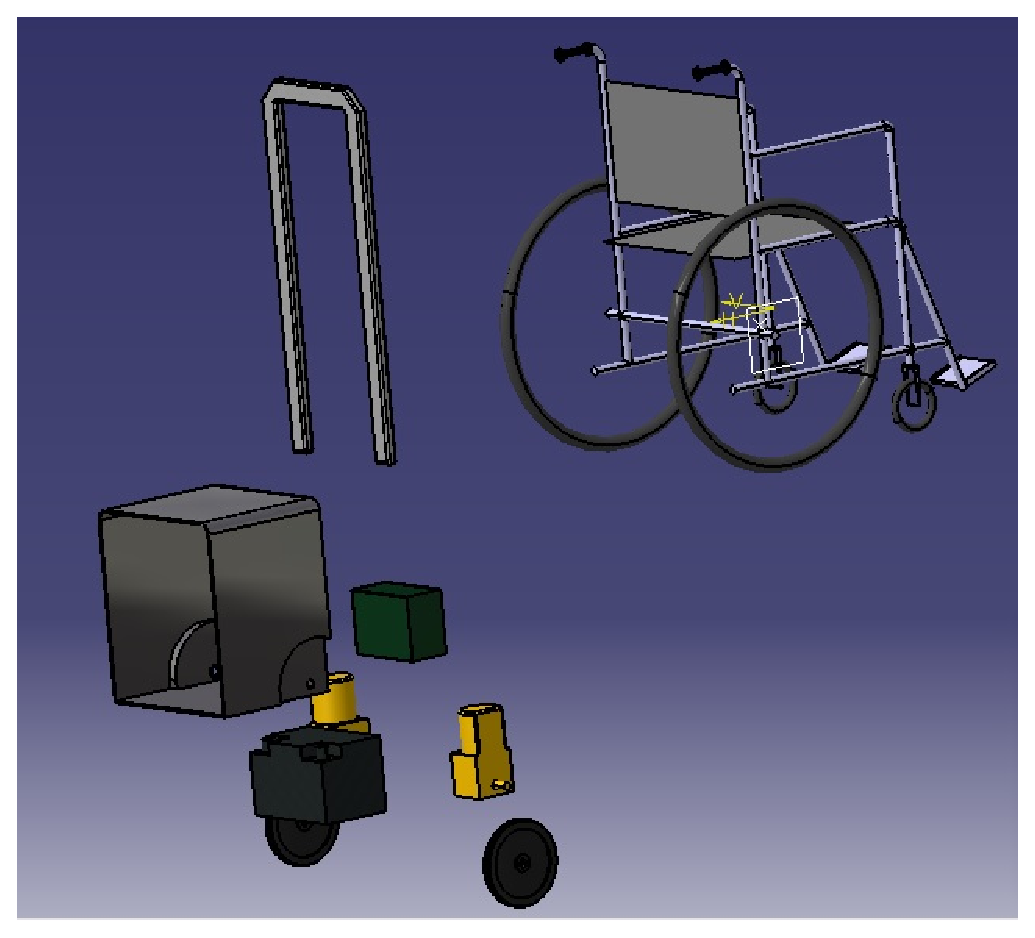
\includegraphics[keepaspectratio=true,scale=0.4]{figuras/estrutura/explode}
\caption{Visão do Sistema}
\label{fig:sistema}
\end{figure}

Cada roda possuirá um motor próprio para que seja possível rotaciona-lás em sentidos opostos, por exemplo, quando for necessário fazer manobras em que a rotação deve ocorre em torno do eixo do próprio cadeirante, movimento muito comum para manobrar uma cadeira de rodas. Assim o cadeirante se sentira confortável e não terá grandes dificuldades quando for manobrar a cadeira, já que a lógica de controle será a mesma usada quando se propulsiona manualmente a cadeira.

\begin{figure}[!htb]
\centering
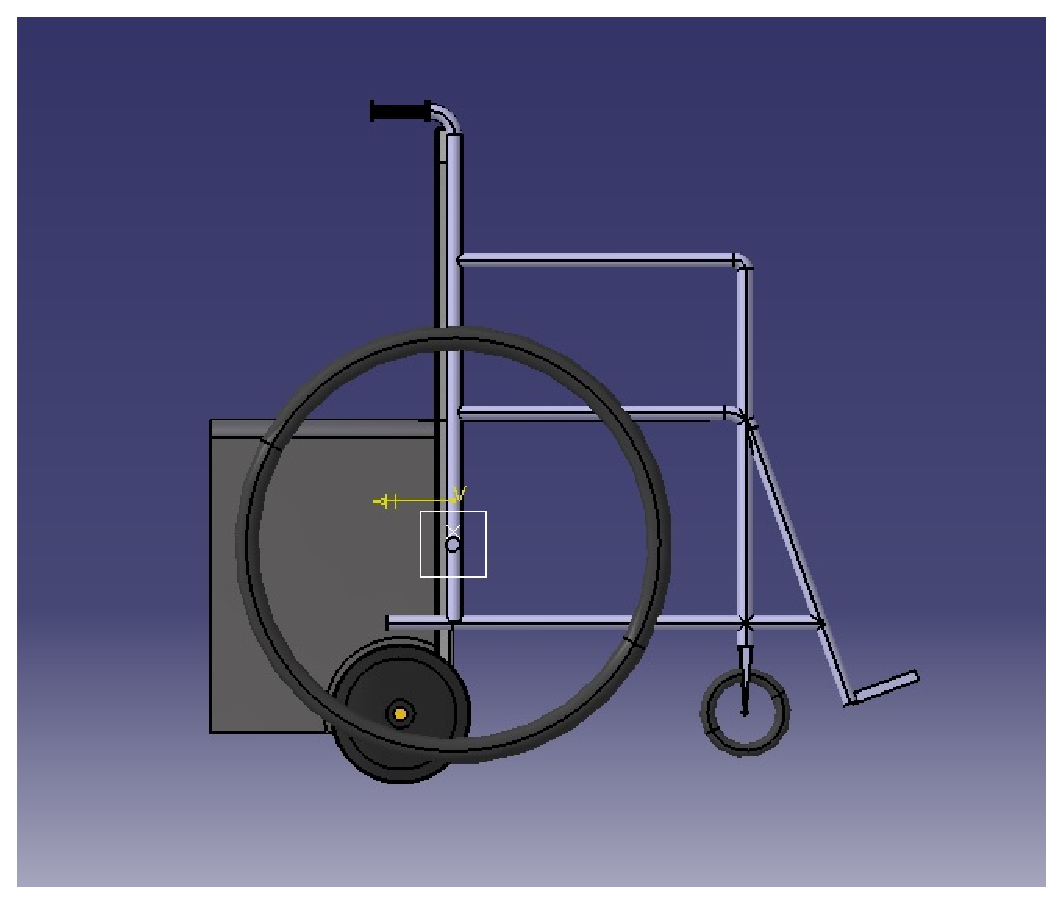
\includegraphics[keepaspectratio=true,scale=0.4]{figuras/estrutura/vista_lateral_cadeira}
\caption{Imagem Lateral}
\label{fig:lateral}
\end{figure}

Como pode se notar nas figuras, o sistema de propulsão devera empurrar a cadeira de rodas, pois assim podemos aproximar o máximo possível o eixo da roda que ira gerar o movimento ao eixo da maior roda da cadeira, o que diminui a quantidade de torque necessário para movimentar o conjunto, fazendo com que o consumo de energia diminua e possibilite o uso de um motor de menor potencia, que diminuirá o custo do produto final.

\begin{figure}[!htb]
\centering
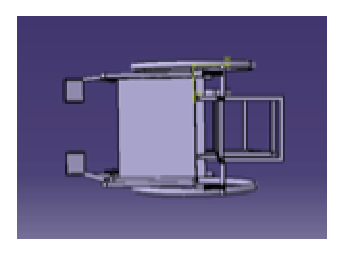
\includegraphics[keepaspectratio=true,scale=0.4]{figuras/estrutura/vista_superior}
\caption{Imagem Superior}
\label{fig:superior}
\end{figure}

\section{Power Train}
\subsection{Motor}

Será utilizado no projeto o motor de corrente contínua. A escolha foi feita pois esse tipo de motor é muito utilizado em projetos que necessitam de velocidades variáveis, eles também apresentam uma região de torque e potência constante e são simples de realizar a aceleração e a desaceleração \cite{manual_bateria_unipower}.

Especificações a serem atendidas:
\begin{itemize}
 \item Velocidade máxima de 7,2 km/h apx: 2m/s;
 \item Peso máximo de 120 kg;
 \item Peso da bateria 10 kg;
 \item Peso da cadeira (valor aproximado) 20kg;
 \item Peso total estimado: 150 Kg;
 \item Considerando hipoteticamente o coeficiente de atrito ($\mu$): 0,2.
\end{itemize}

\textbf{Força de atrito:}
\begin{equation}
 \overrightarrow{F} = \overrightarrow{N} * \mu = 150 * 9,8 * 0,2 = 294N
\end{equation}

\textbf{Potência do motor:}

\begin{equation}
 P_{x} = \frac{F * v}{100} = \frac{294 * 2}{1000} = \frac{588}{100} = 0,588kW
\end{equation}

O motor para a utilização na aplicação deve seguir algumas características dentro das especificações do projeto. Serão utilizados dois motores para motorizar a cadeira de rodas. Com isso é necessário que cada motor tenha a potência mínima de: \textbf{294W}.

\subsection{Baterias}
A bateria de chumbo-ácido é muito utilizada hoje em dia em diferentes áreas,  como automóveis, sistemas de fornecimento de energia elétrica ininterrupta (no-breaks) e cadeiras de rodas elétricas. Desprezando-se o problema do peso e considerando as observações feitas anteriormente no capítulo \ref{cap:fundamentacao_teorica} foi a bateria escolhida para o projeto, considerando ainda o seu fácil acesso e baixo  custo.

\subsubsection{Autonomia}

A capacidade de armazenamento de energia de uma bateria é medida através da multiplicação da corrente de descarga pelo tempo de autonomia, sendo dado em Ampére-hora (Ah). Cálculo da autonomia da bateria em horas:

$Autonomia(h) = \frac{Capacidade da bateria(Ah)}{Consumo do circuito(A)}$
Potencia é dada por:
\begin{equation}
 P=U*I
\end{equation}

Para o projeto são necessários dois motores de no mínimo 294W de potência cada, ou seja, os dois motores terão, em conjunto, uma potência de 588W. Os motores a serem utilizados vão operar a uma tensão de 12V, com isso a corrente necessária é de:
\begin{equation}
588 [W] = 12 [V] * I [A]
\end{equation}

\begin{equation}
I = \frac{588}{12} = 49A
\end{equation}

\section{Controle}

O kit de automação para cadeiras de roda será e um produto projetado para auxiliar na locomoção do cadeirante em um shopping. Na Figura \ref{fig:esquema_controle} foi feita uma proposta de construção do kit mostrando a sua estrutura de controle. Em verde claro tem-se um componente que talvez seja somente integrado ao sistema. Esses blocos foram resultado dos estudos teóricos e de discursões da equipe. Em verde escuro, sistemas que serão efetivamente projetados e construídos e em azul, componentes que não serão construídos mas farão parte do kit de automação.

\begin{figure}[!htb]
\centering
  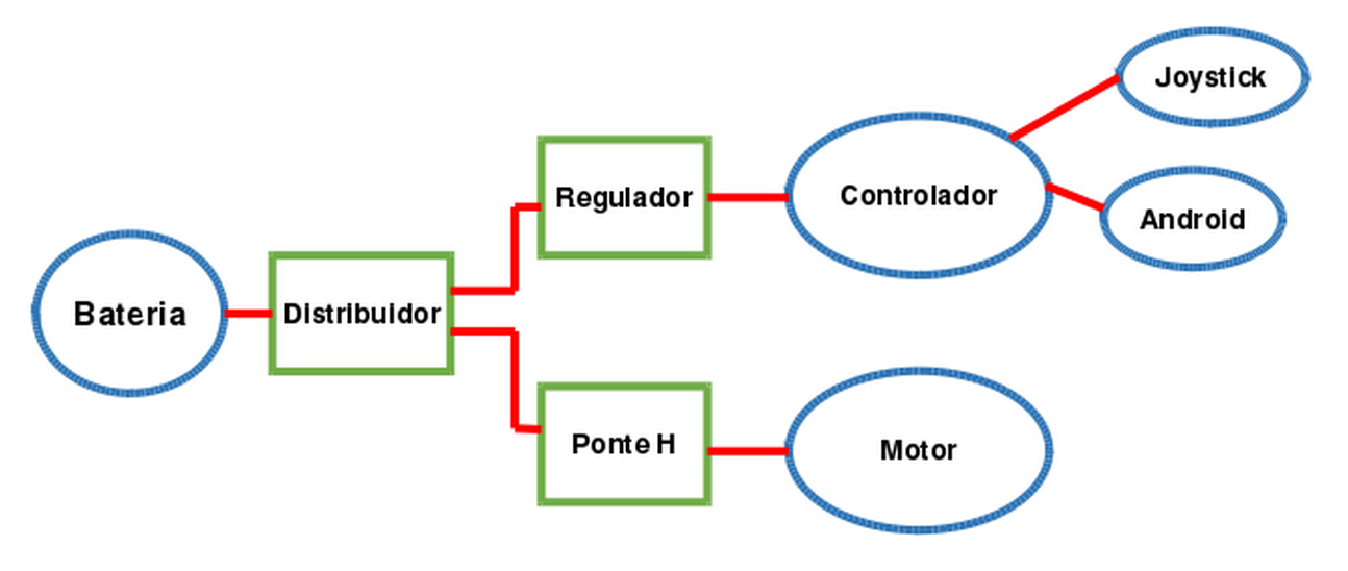
\includegraphics[keepaspectratio=true,scale=0.6]{figuras/controle/esquema_controle}
\caption{Esquemático de funcionamento geral da cadeira de rodas automatizada}
\label{fig:esquema_controle}
\end{figure}


Para o kit de automação da cadeira de rodas, será utilizada a ponte H para o controle dos motores. Um algoritmo de controle PWM usando o Raspeberry Pi que deve responder aos comandos do usuário como direção, aceleração, frenagem, entre outros que serão posteriormente levantados. Na figura \ref{fig:diagrama_blocos} pode ser obervado o esquemático geral do sistema. Tem-se ainda o Distribuidor, uma placa para facilitar a alimentação do sistema, e o Regulador, para alimentar o Controlador e periféricos.

\begin{figure}[!htb]
\centering
  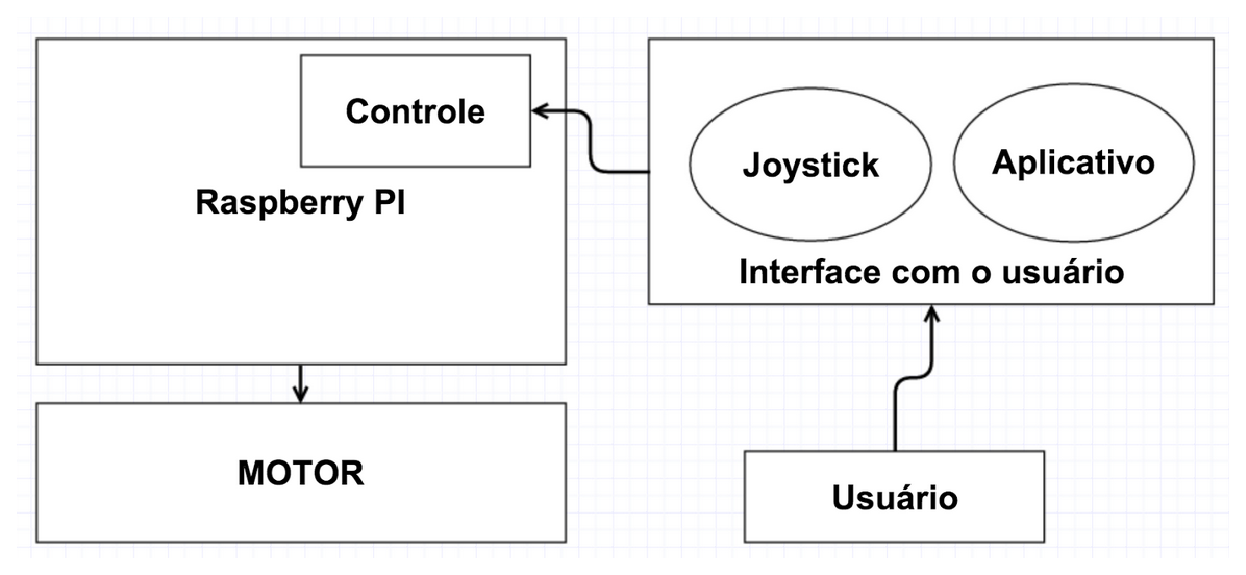
\includegraphics[keepaspectratio=true,scale=0.6]{figuras/controle/diagrama_blocos}
\caption{Desenho do diagrama de blocos do sistema de controle}
\label{fig:diagrama_blocos}
\end{figure}

O sistema vai ser projetado de forma que não seja necessário retirar a bateria para essa ser carregada, o grupo ainda não estabeleceu se o carregador vai ser construído ou comprado, considerando que o tempo disponível para o desenvolvimento do projeto é relativamente curto.

O Distribuidor vai ser basicamente uma placa que facilitara a conexão de todas as outras ao sistema, assim não será necessário que haja reduções de tensão tão drásticas. A placa terá um circuito de proteção, para evitar problemas de sobretensão e curto, saídas para a ponte H, tanto para alimentar possíveis circuitos e motor e ainda saídas para o regulador.

O Regulador terá a funcionalidade de alimentar o controlador com seus periféricos. Essa placa terá um circuito de proteção, para o controlador, contra possíveis problemas do distribuidor, saídas de alimentação para o controlador e ainda uma USB de alimentação para o celular do usuário, para impedir problemas de falta de bateria.

A ponte H será o circuito responsável por fazer o controle de velocidade e direção dos motores. Essa placa terá além dos circuitos necessários para o funcionamento da ponte H, um circuito de proteção para os motores e pinos de entrada do PWM, já que pode haver possíveis problemas de sobretensão a alimentação do motor.


\section{Interface com o usuário}


\subsection{Joystick}
Para as cadeiras de rodas automatizadas essa é uma solução comum de controle para as mesmas, tendo em vista que é relativamente simples de ser acoplado uma vez que se entenda seu funcionamento básico. Para o projeto em questão essa foi uma das alternativas encontradas. No qual o joystick seria acoplado ao braço da cadeira, ou em uma posição que o usuário se sinta mais ergonomicamente confortável. Este acoplamento deve ser simples para favorecer a característica de portabilidade do projeto como um todo.

Caso necessário a conexão do joystick ao sistema de controle pode ser feita por bluetooth, tal característica contribui para o objetivo final do projeto \cite{artigo_joystick_controller}.

\subsubsection{Smartphone}
O \textit{smartphone} é um telefone celular com um sistema operacional móvel avançado que combina as características de um sistema operacional de computador pessoal com outros recursos úteis para uso móvel ou portátil \cite{article_smartphone}.

Devido a portabilidade destes dispositivos e sua facilidade de integração com outros sistemas, uma possível solução para a interação do usuário com o sistema pode ser feita. Uma conexão entre o dispositivo e o sistema será feita através de Bluetooth (Android) ou "Virtual Private Network" (iOS e Android). Para o projeto em questão o usuário pode optar por utilizar o \textit{Smartphone} ou ainda o joystick.

\subsubsection{Protótipo}

O protótipo na figura \ref{fig:prototipos} foi feito com o intuito de mostrar o fluxo do aplicativo sugerido para o controle da cadeira de rodas automatizada.

A principal funcionalidade deste aplicação é basicamente voltada para o controle da cadeira de rodas automatizada, no qual o usuário teria um \textit{joystick} virtual que se comunica com o \textit{Raspeberry Pi} enviando o comando para os motores.
Uma das restrições pensadas, foi a de enquanto o controle estiver ativado via aplicativo o usuário não poderia ter o controle através do \textit{joystick} físico.


  \begin{figure}[!htb]
		\centering
		\legend{}
    \subfloat{
  		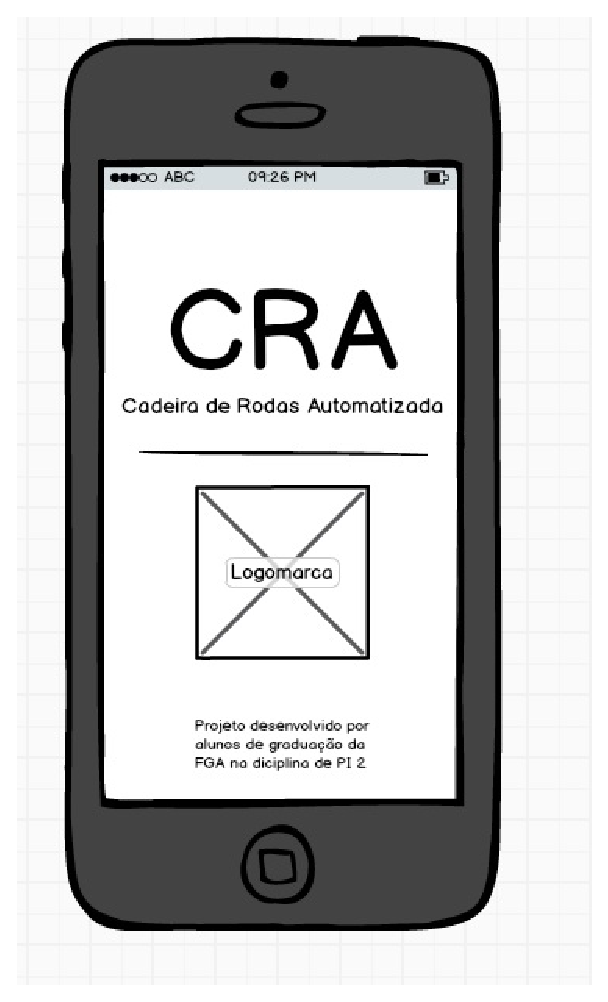
\includegraphics[keepaspectratio=true,scale=0.6]{figuras/controle/tela_1}
		}
		\quad %espaco separador
		\subfloat{
  		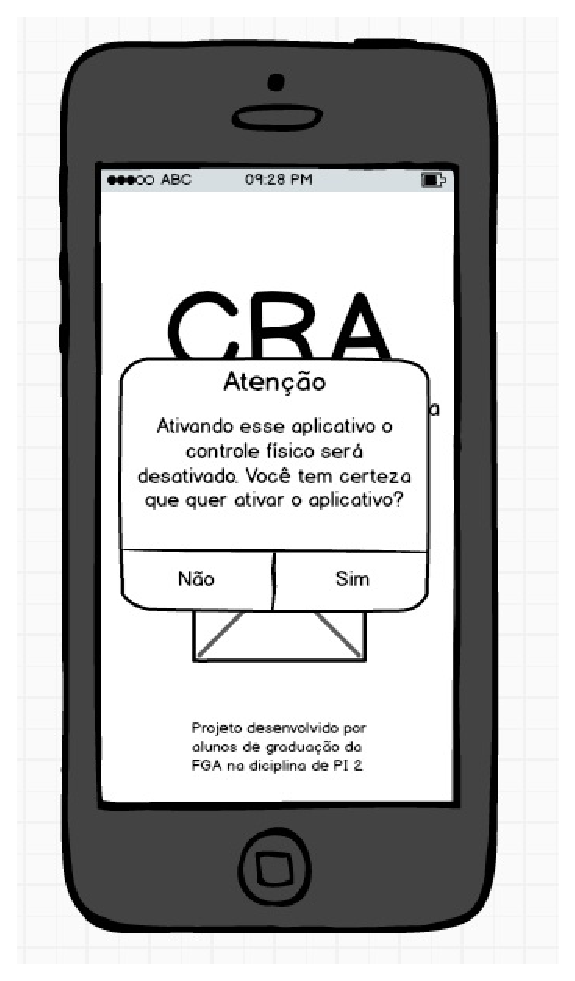
\includegraphics[keepaspectratio=true,scale=0.6]{figuras/controle/tela_2}
		}
		\subfloat{
  		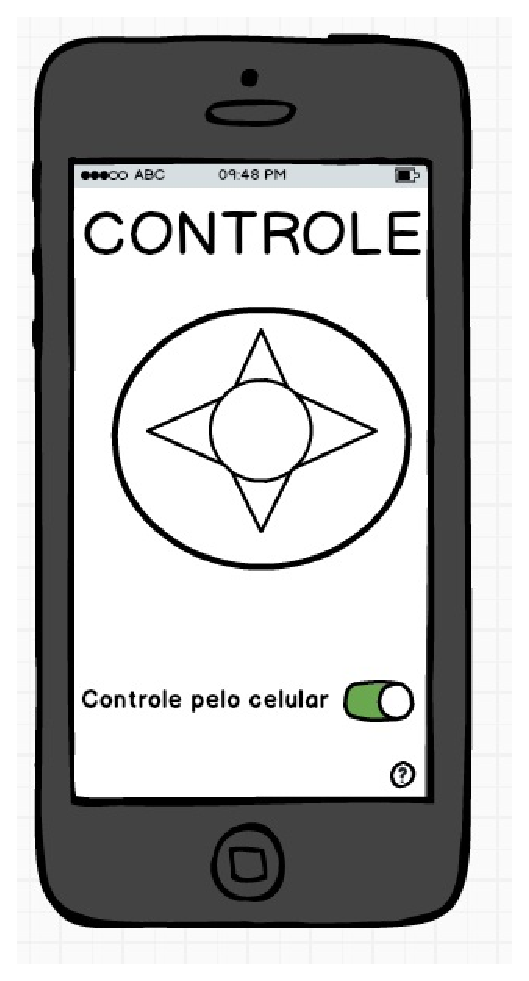
\includegraphics[keepaspectratio=true,scale=0.6]{figuras/controle/tela_3}
		}
		\quad %espaco separador
		\subfloat{
  		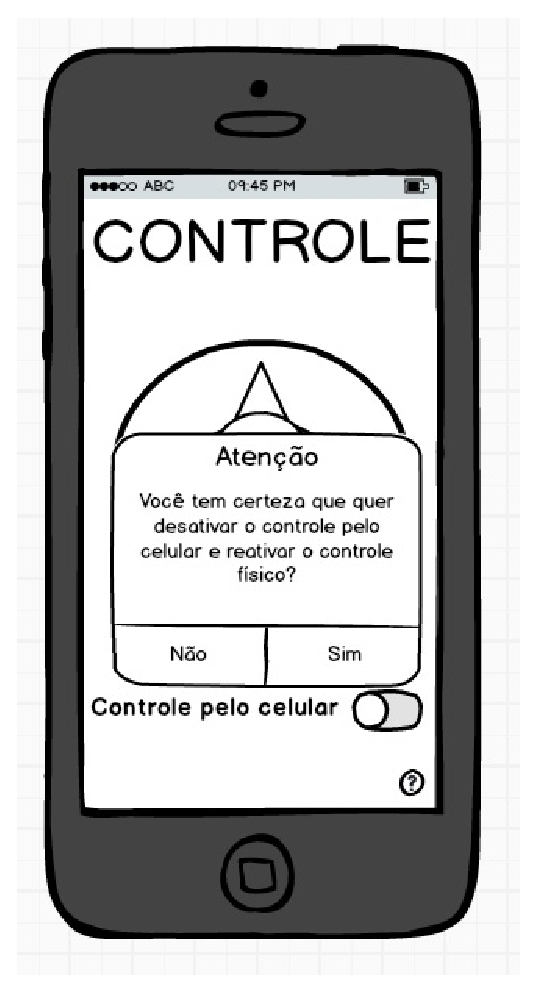
\includegraphics[keepaspectratio=true,scale=0.6]{figuras/controle/tela_4}
		}
		\caption{Protótipo de aplicativo para interface entre usuário e motor}
		\label{fig:prototipos}
  \end{figure}
